\chapter{Variable Gear-ratio Actuation }
\label{sec:MultipleSpeedActuationTechnology}

This chapter present an actuation technology, consisting of a mechanical architecture called DSDM (dual-motor dual-speed) used in conjunction with novel gear-shifting control algorithms. 

\section{Motivation}
\label{sec:mot}

In many robotic systems, actuators are often required to operate in distinctively different torque-speed load conditions. A legged robot, for example, has to move its leg forward quickly through the air and, once touching the ground, it has to bear a large load \cite{hirose_study_1984}. These two operating conditions, high speed at low torque vs. high torque at low speed, are often an order of magnitude different, while the required output power is similarly low. When the torque-speed load conditions do not vary significantly, a single gear ratio can be picked so that the actuator always operate under nearly optimal conditions. For distinctively different torque-speed conditions, the actuator will be far for its optimal operating conditions with a gear ratio picked from the middle ground. As illustrated on Fig. \ref{fig:speedissue} for a typical electromagnetic (EM) actuator, extremum torque-speed conditions are not optimal in term of efficiency and power output. 

\begin{figure}[htp]
	\centering
		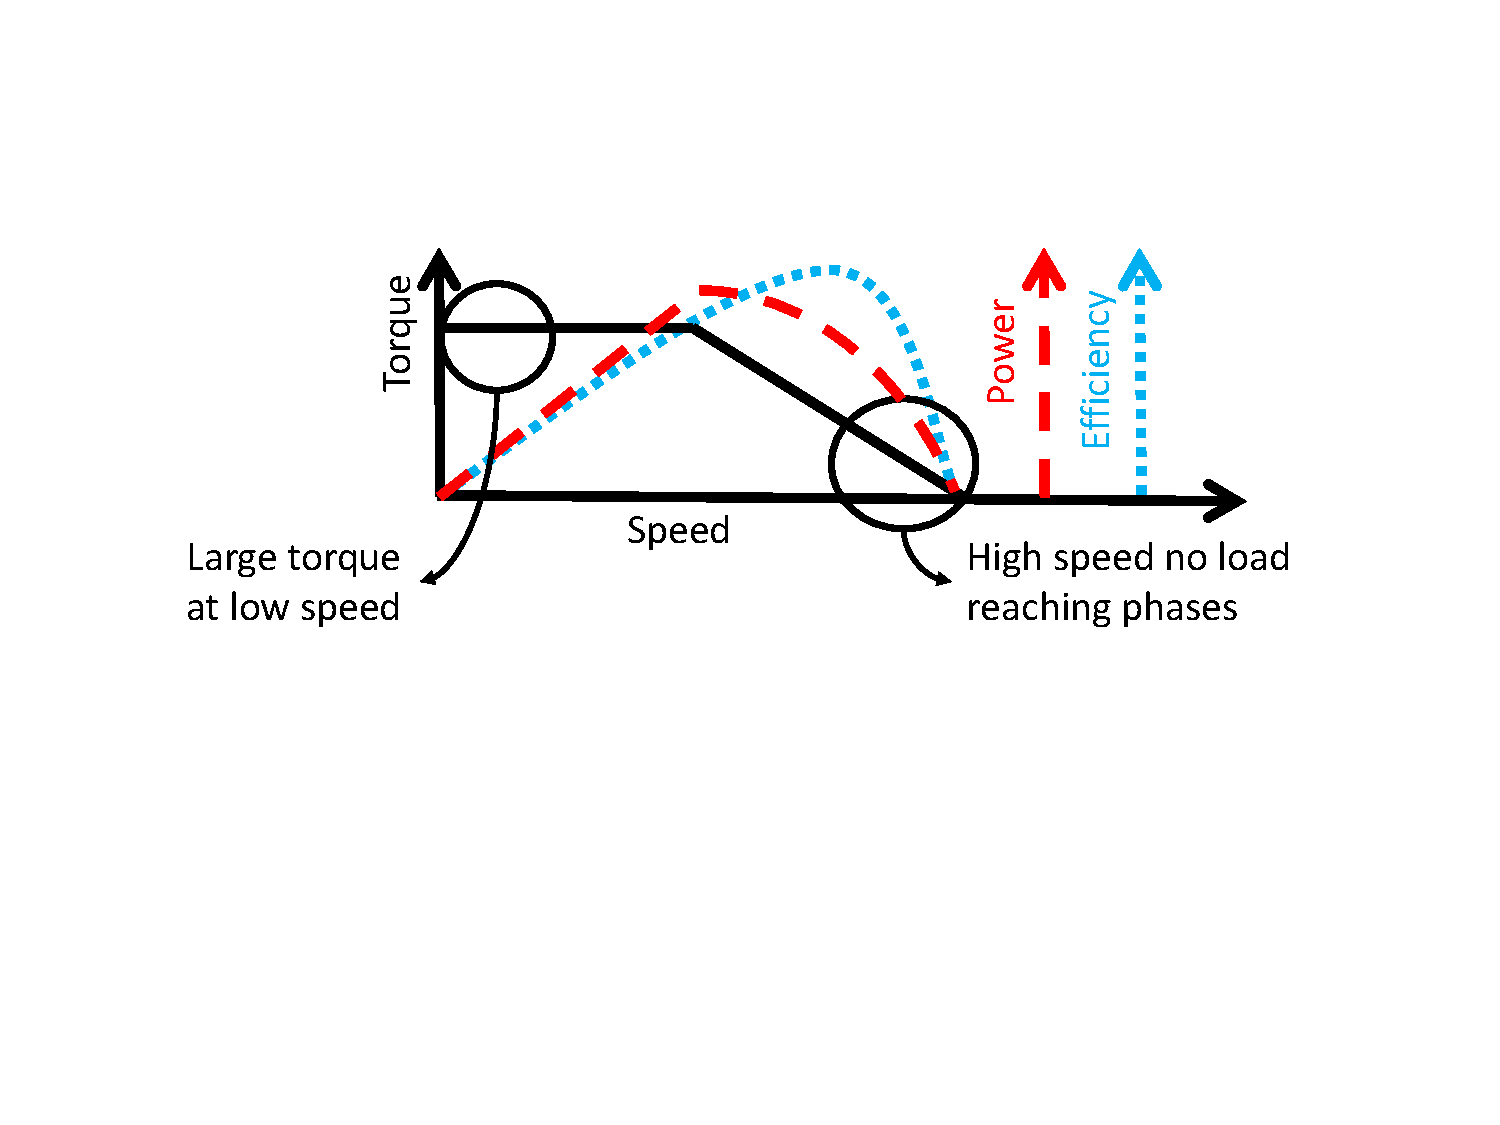
\includegraphics[width=0.70\textwidth]{speedissue.pdf}
	\caption{Limitations of EM motors for extremum torque-speed operations}
	\label{fig:speedissue}
\end{figure}

EM motors cannot output high power at low speed because of thermal dissipation and magnetic flux limits related to material properties; are limited in speed by the supply tension and others; and are very inefficient when producing large forces at low speed \cite{hollerbach_comparative_1992}. This often leads to the use of oversized and inefficient actuators, which is inhibitory particularly for mobile robots.

Automobiles with internal combustion (IC) engines use transmissions with multiple gear ratios to match torque-speed conditions. IC engines have a very narrow speed range in which they can effectively deliver power; a transmission with multiple gear ratios is a necessity for the engine to work effectively for a wide range of output speed. EM motors are more flexible than IC engines, but still far from ideal sources. EM motors cannot output high power at low speed because of thermal dissipation and magnetic flux limits related to material properties; are limited in speed by the supply tension and others; and are very inefficient when producing large forces at low speed \cite{hollerbach_comparative_1992}. In robotic, since it is often the extremums, i.e. maximum torque and speed, that determine the actuator design instead of the power requirement, much can be gained with multiple gear ratios.

It will be a significant breakthrough if a type of multiple speed transmission can be used effectively in robotics. Even a small, lightweight actuator can generate large torques and move at high speed if equipped with both large and small gear ratio. Moreover, multiple speed transmission can allow an actuator to work closer to its optimal operating conditions, improving overall efficiency significantly. Furthermore, gear shifting significantly changes the intrinsic impedance of an actuator, since the impedance is proportional to the square of gear ratio. The actuator may be made back-drivable while using its small reduction ratio, an important property in many applications where the robot physically interacts with the environment \cite{hogan_impedance_2004}. Also the same actuator may be made non-back-drivable while using its large reduction ratio, allowing the actuator to support loads without consuming energy and enabling high-stiffness position control.



\section{Actuator Research}
\label{sec:actres}

Traditional robots generally use actuators that behave as displacement-sources because of their high intrinsic impedance. These include geared EM motors and hydraulics cylinders. Using a force sensor, it is possible to control the output force using those actuators, but the bandwidth is rather limited. To guarantee the stability of the force-feedback scheme only half the intrinsic inertia can be canceled \cite{hogan_impedance_2004}. Since 70's, roboticists have been attempting to build actuators that can behave naturally as a force-source such as series-elastic actuators, pneumatic cylinder and air-muscles \cite{hanafusa_stable_1977}\cite{pratt_series_1995}. However, because of the physical limitation of compliant transmission materials, the achievable bandwidth is limited and precise position control is hardly achievable. Direct drive EM actuators are the best force-source actuators with high fidelity, high bandwidth. However, the very low force density and low efficiency at low speeds make them impractical for mobile robot applications \cite{hollerbach_comparative_1992}. Moreover, on the other hand, actuators with non-back-drivable mechanisms have the advantage for pure position control tasks and they can bear very large load without any power consumption.

Since both small and large intrinsic impedances are advantageous in different scenario, several group have developed variable intrinsic impedance actuators, such as based on variable stiffness spring \cite{tonietti_design_2005}, antagonist non-linear devices \cite{koganezawa_antagonistic_2006}, a series-compliance that can be locked with a brake \cite{leach_linear_2012} and dual-motors in serial configuration \cite{kim_serial-type_2010}. Furthermore, so-called macro-micro actuators, can improve the bandwidth of force-source type of actuators by exploiting the high-bandwidth of a small actuator in parallel, allowing for wider-range impedance control and improved position control \cite{morrell_parallel-coupled_1998}.

While the actuator work in robotics have been focused on impedance and bandwidth issues, in the powertrain field the torque-speed matching issue is predominant, since power density and efficiency are critical for mobile systems. The idea of using multiple gear ratios with electric motors has been explored occasionally, to improve efficiency and power density \cite{mckeegan_antonovs_2011}. A twin motor configuration has been proposed for smooth gear shifting, where each motor shifts at a different timing \cite{bologna_electric_2014}. Also, a dual motor configuration using a planetary coupling and non-back-drivable worm-gears was proposed for a mobile robot powertrain \cite{lee_new_2012}. Multiple speed powertrains provide effective solutions for torque-speed matching, but are not adapted to make gear shifts while interacting with dynamic environment and a new gear shifting methodology adapted to robotics is needed.

This presented actuator work in this chapter, address the issue of improving available power and efficiency over a wide range of operating speeds, which has rarely been addressed in the robotics literature. Also, the proposed dual-speed actuator is an alternative approach to impedance variation that can achieve many order-of-magnitude changes. The main novel contribution is the methodology for gear shifting that is adapted to a robotics context. A mechanical architecture where two motors are coupled using a 3-ports gearbox and a brake is used. Similar dual-motor architectures have been used in hybrid car powertrains and actuators \cite{byeong-sang_kim_improved_2007}, but not in a the context of addressing gear shifting issues, i.e. the control of transitions between discrete operating modes. Here this architecture is used in conjunction with a novel controller to provide full control of the output during gear shifting, which is a key enabling feature for robotic applications.


\section{Dual-Speed Dual-Motor architecture}
\label{sec:DSDM}

The proposed architecture, referred to as a Dual-Speed Dual-Motor (DSDM) actuator, consists of a direct drive motor (M1) equipped with a locking brake and an geared EM motor (M2) with a large reduction ratio coupled to the same output through a differential, see Fig. \ref{fig:dualmotorconcept}. The differential can be viewed as a 0-type junction (taking bond-graph terminology) where the speeds add up and the force is shared. 


\begin{figure}[H]
	\centering
		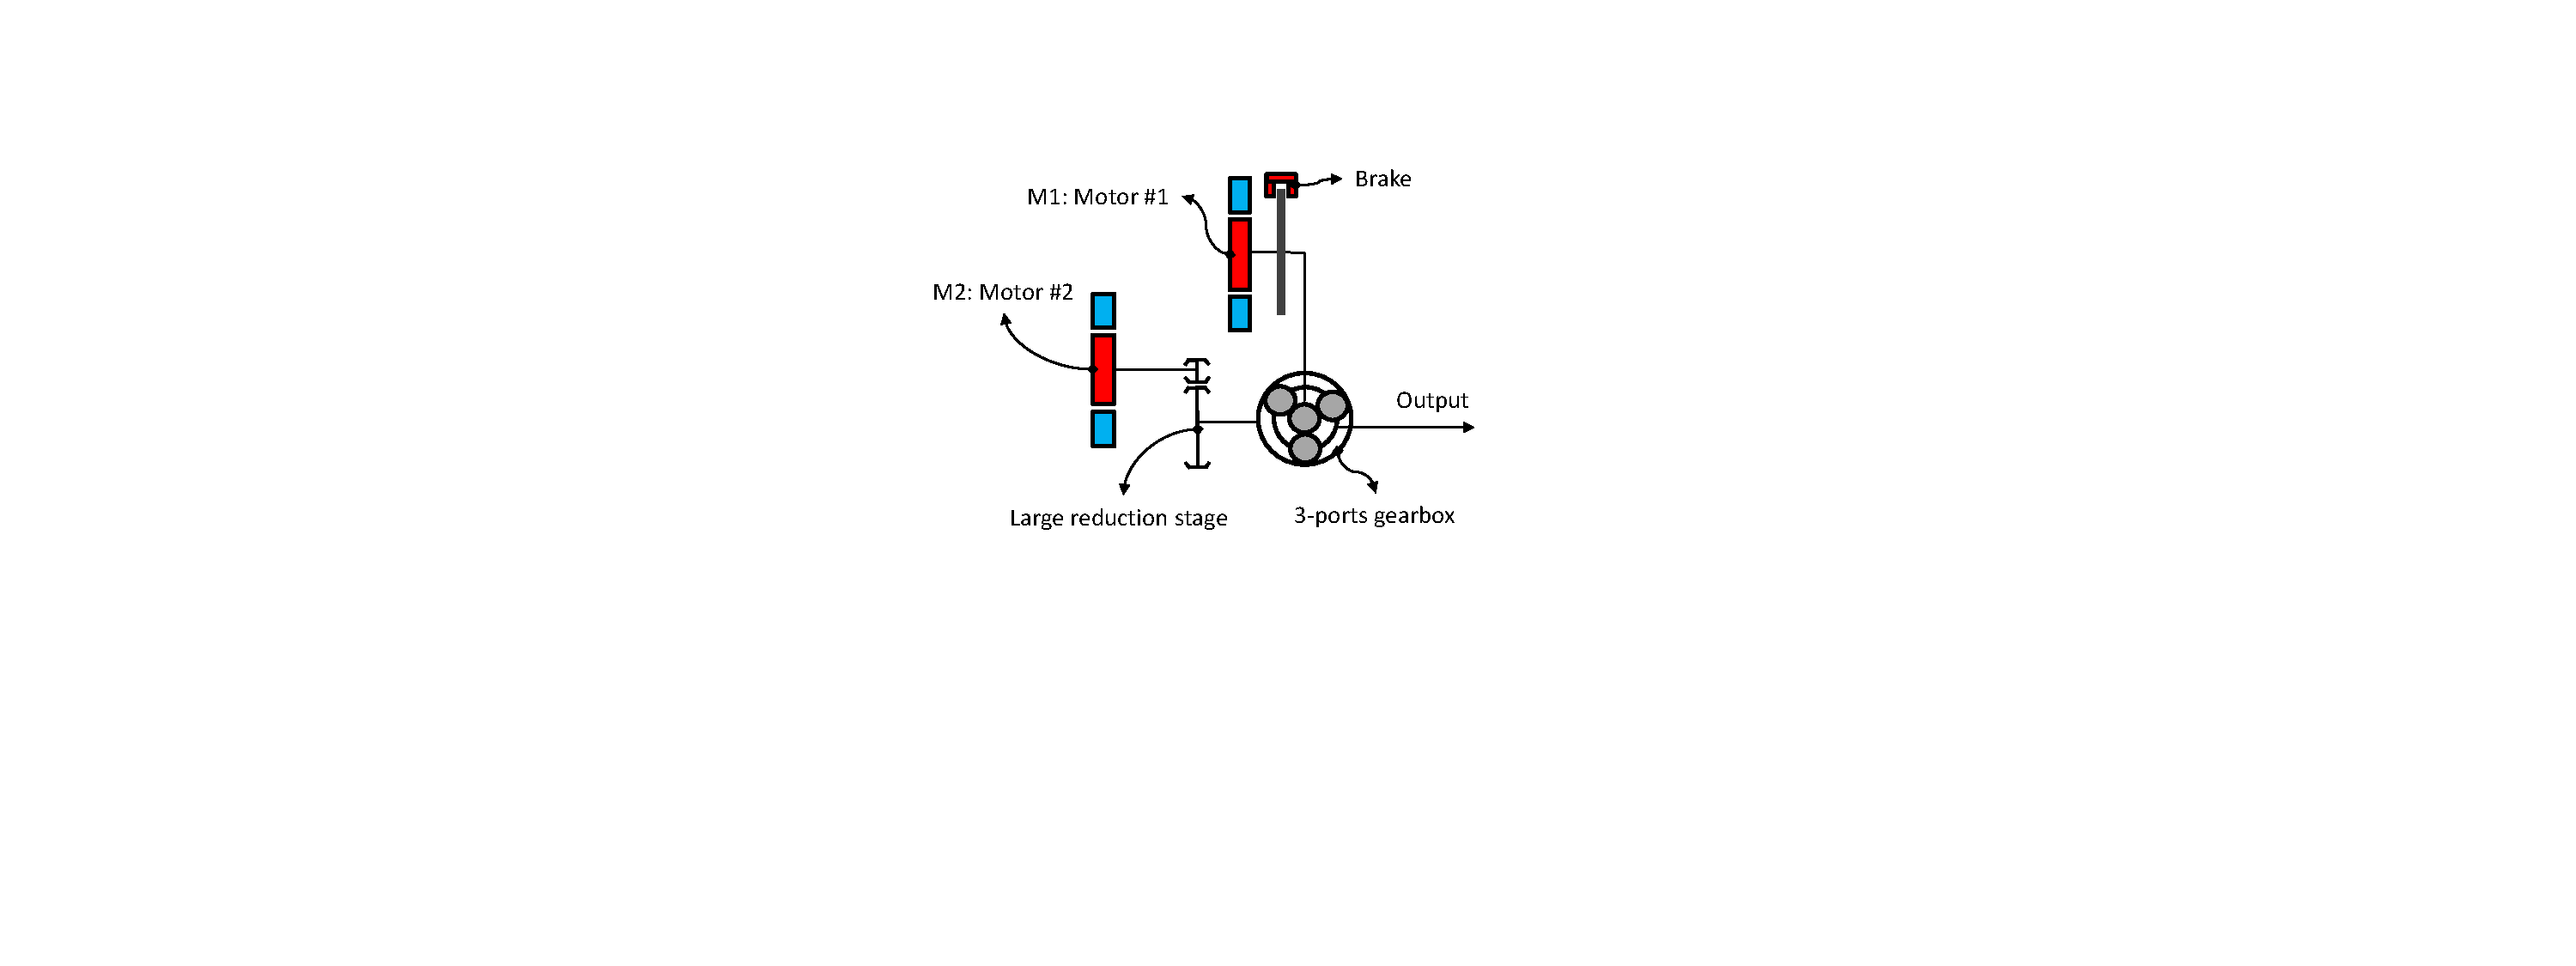
\includegraphics[width=0.60\textwidth]{dualmotorconcept2.pdf}
	\caption{DSDM actuator concept}
	\label{fig:dualmotorconcept}
\end{figure}

The envisioned implementation of the DSDM concept is to embed all the components into a single compact unit, as illustrated by Fig. \ref{fig:embedded}. A lot of weight and space could be saved by combining the reduction and the differential gearing and having all the components inside a single housing. 


\begin{figure}[H]
	\centering
		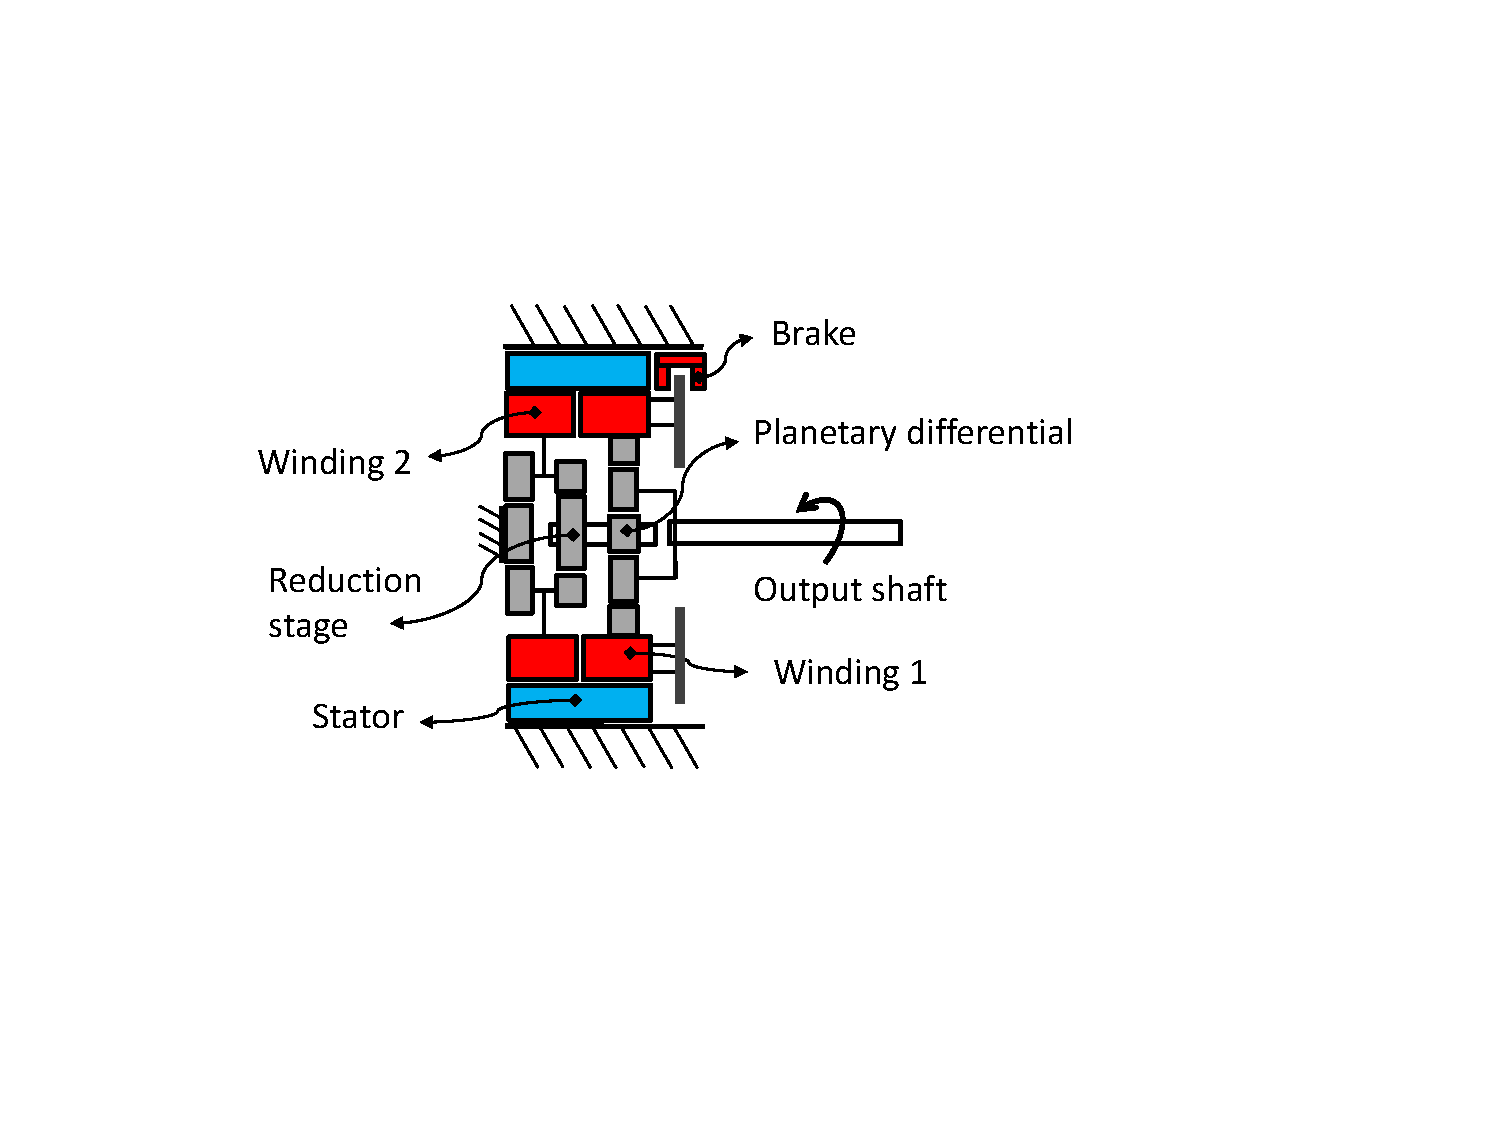
\includegraphics[width=0.60\textwidth]{embedded3.pdf}
	\caption{Possible architecture of an integrated DSDM concept}
	\label{fig:embedded}
\end{figure}

Fig. \ref{fig:embedded} shows a prototype of a DSDM actuator with a revolute output, using discrete off-the-shelf motors for modularity and ease of implementation.

\begin{figure}[H]
	\centering
		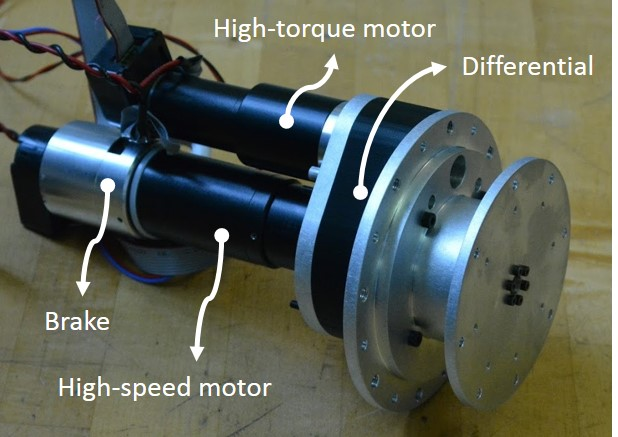
\includegraphics[width=0.60\textwidth]{dsdm_proto_2.jpg}
	\caption{DSDM actuator prototype}
	\label{fig:dsdm_proto}
\end{figure}


\subsection{Principle}
\label{sec:princ}



The DSDM can be used in two modes, high-force mode when the brake is closed and high-speed mode when the brake is open. The result is like having two very different reduction ratio you can choose from during operation. Fig. \ref{fig:lever} conceptually illustrates the principle with a leverage analogy, M1 acts like a force source connected almost directly to the output and M2 acts like a displacement source with a large lever arm relative to the output. 
%
\begin{figure}[H]
	\centering
		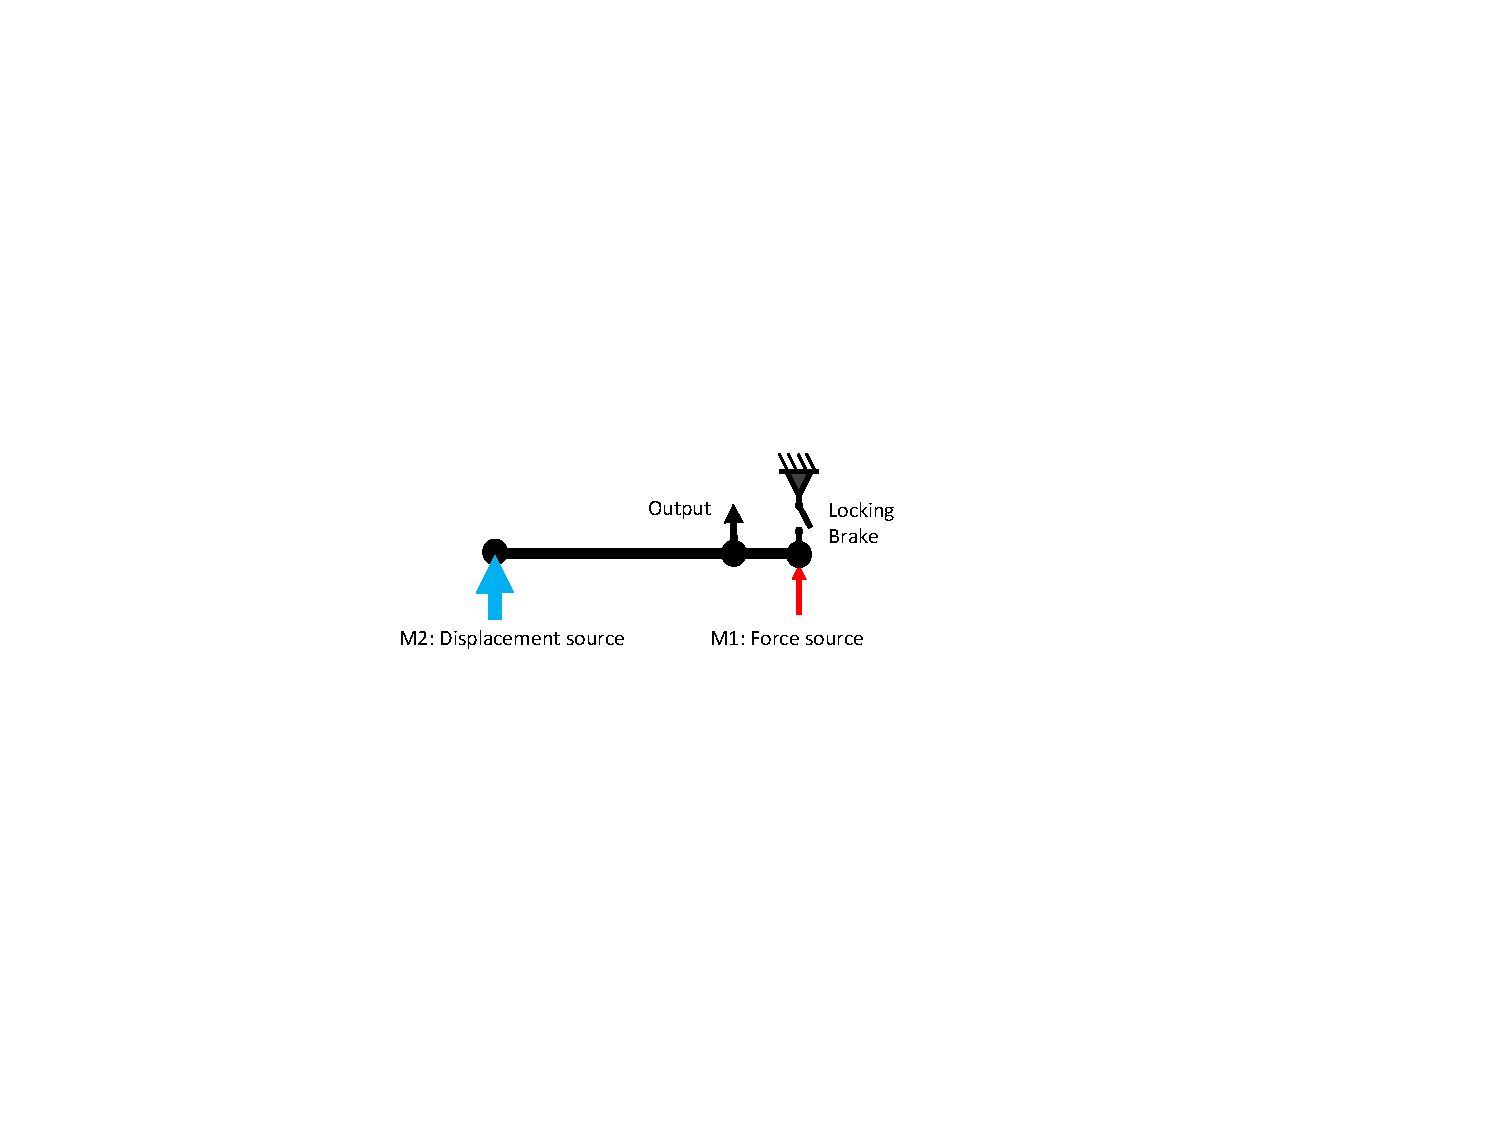
\includegraphics[width=0.60\textwidth]{lever.pdf}
	\caption{Dual input system}
	\label{fig:lever}
\end{figure}
%
During the high-force mode, see Fig. \ref{fig:HF}, the brake is closed and M2 drives the output with a large mechanical advantage. The result is a low-speed displacement-source type of actuation like a geared EM motor. During the high-speed mode, see Fig. \ref{fig:HS}, M1 drive the output almost directly, creating a high-speed force-source actuator like a direct drive EM motor. Additionally, both motors can be used simultaneously to drive the output even faster.
%
\begin{figure}[H]
        \centering
				\subfloat[High force mode (brake closed)]{
        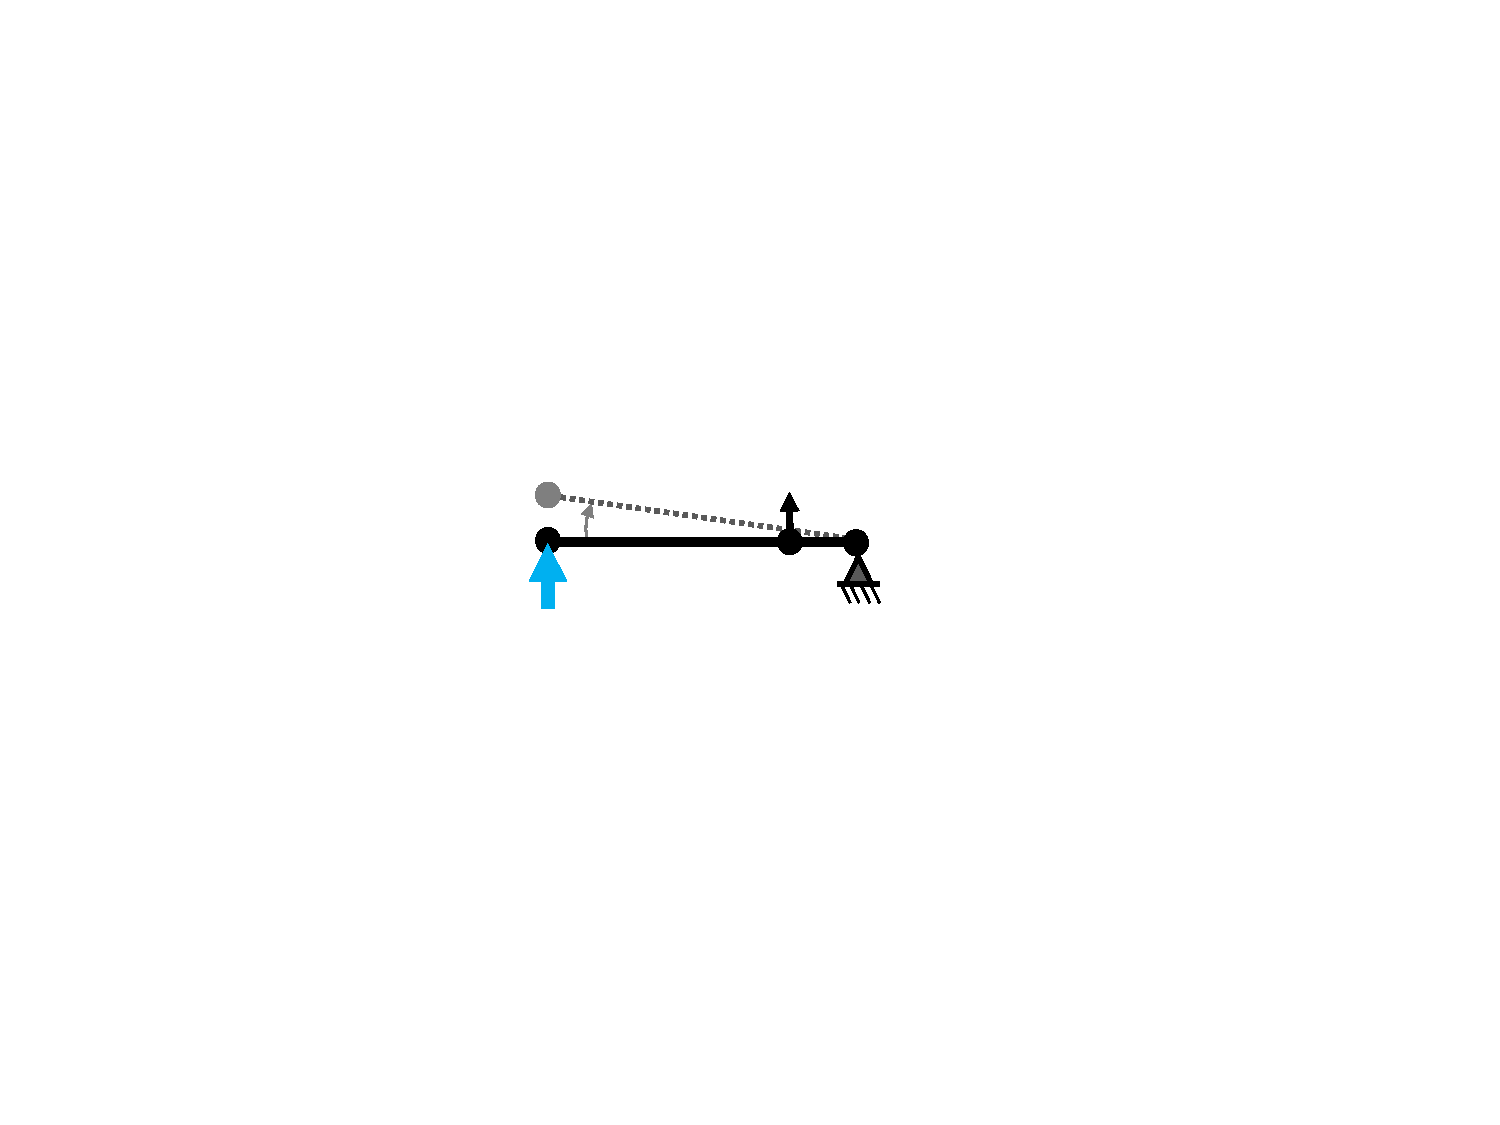
\includegraphics[width=0.38\textwidth]{leverHF.pdf}
				\label{fig:HF}}
        \subfloat[High speed mode (brake open)]{
				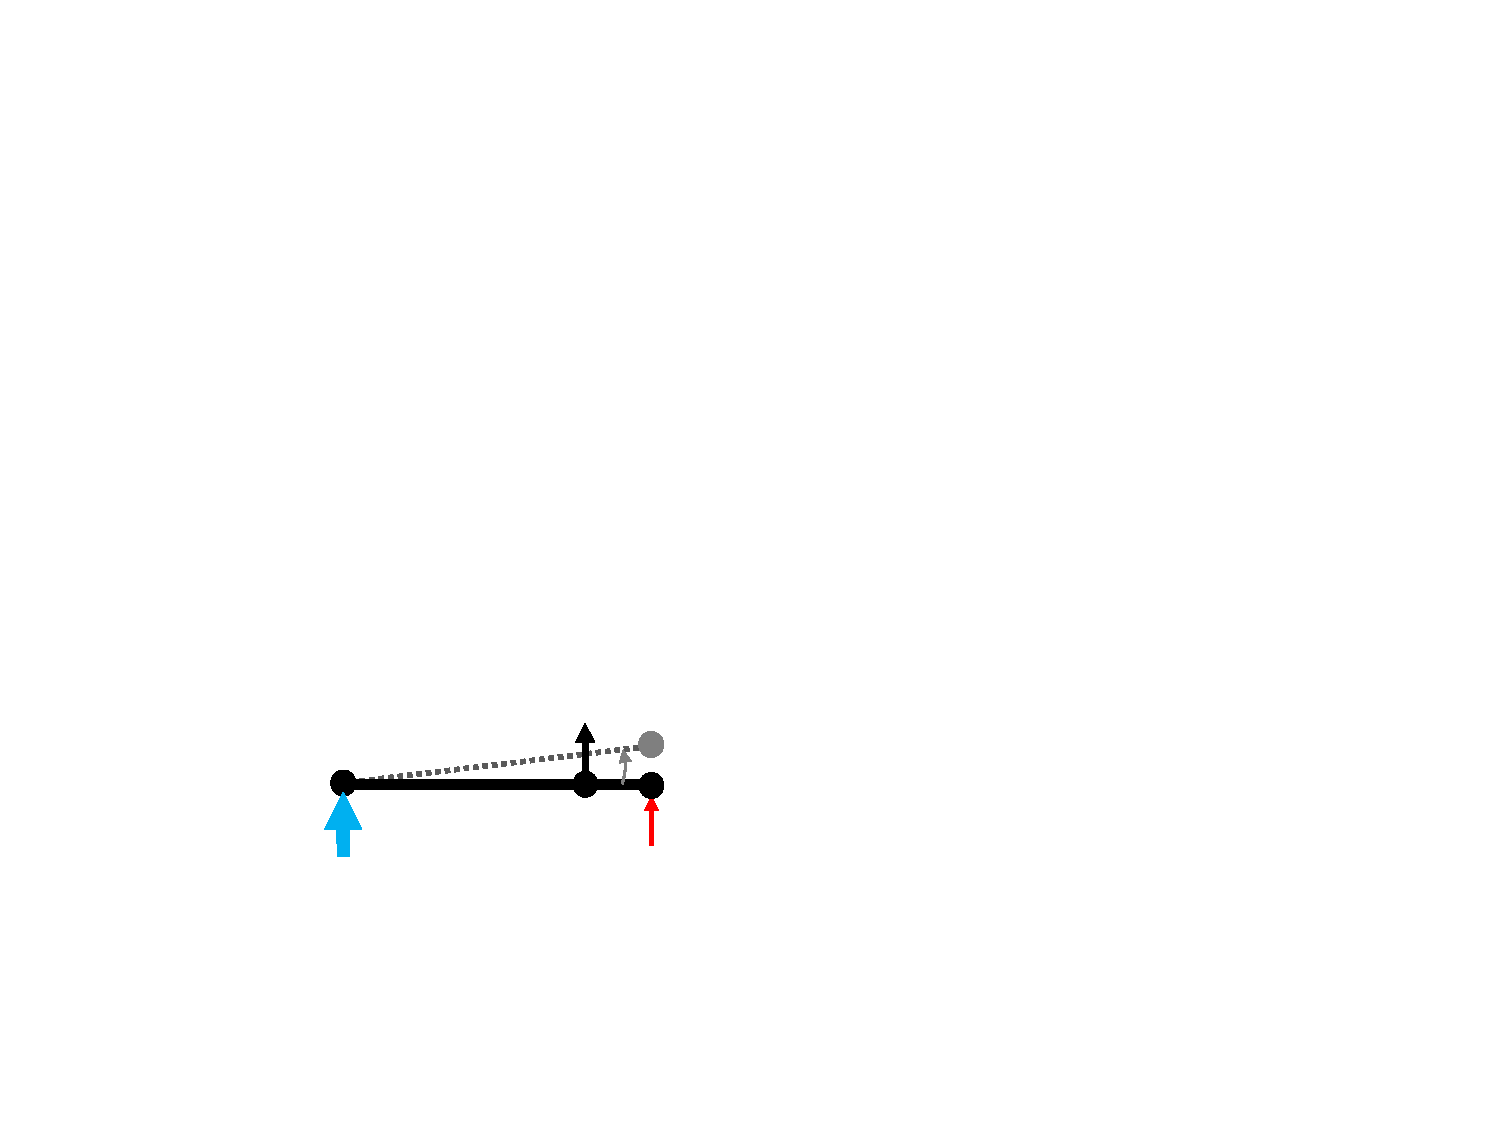
\includegraphics[width=0.38\textwidth]{leverHS.pdf}
				\label{fig:HS}}
        \caption{Two modes of operation}\label{fig:opmode}
\end{figure}

Fig. \ref{fig:torquespeed} illustrates the operating range of the DSDM actuator plotted on the standard torque-speed plane. The high-force mode region is determined by the performance of M2 alone, since M1 is locked. The high-speed mode region can exceed the performance of M1 alone, as M2 can be used simultaneously to increase the output speed. The fail safe zone indicate the guaranteed performance of the DSDM actuator in case of failure in either motor. 

\begin{figure}[H]
	\centering
		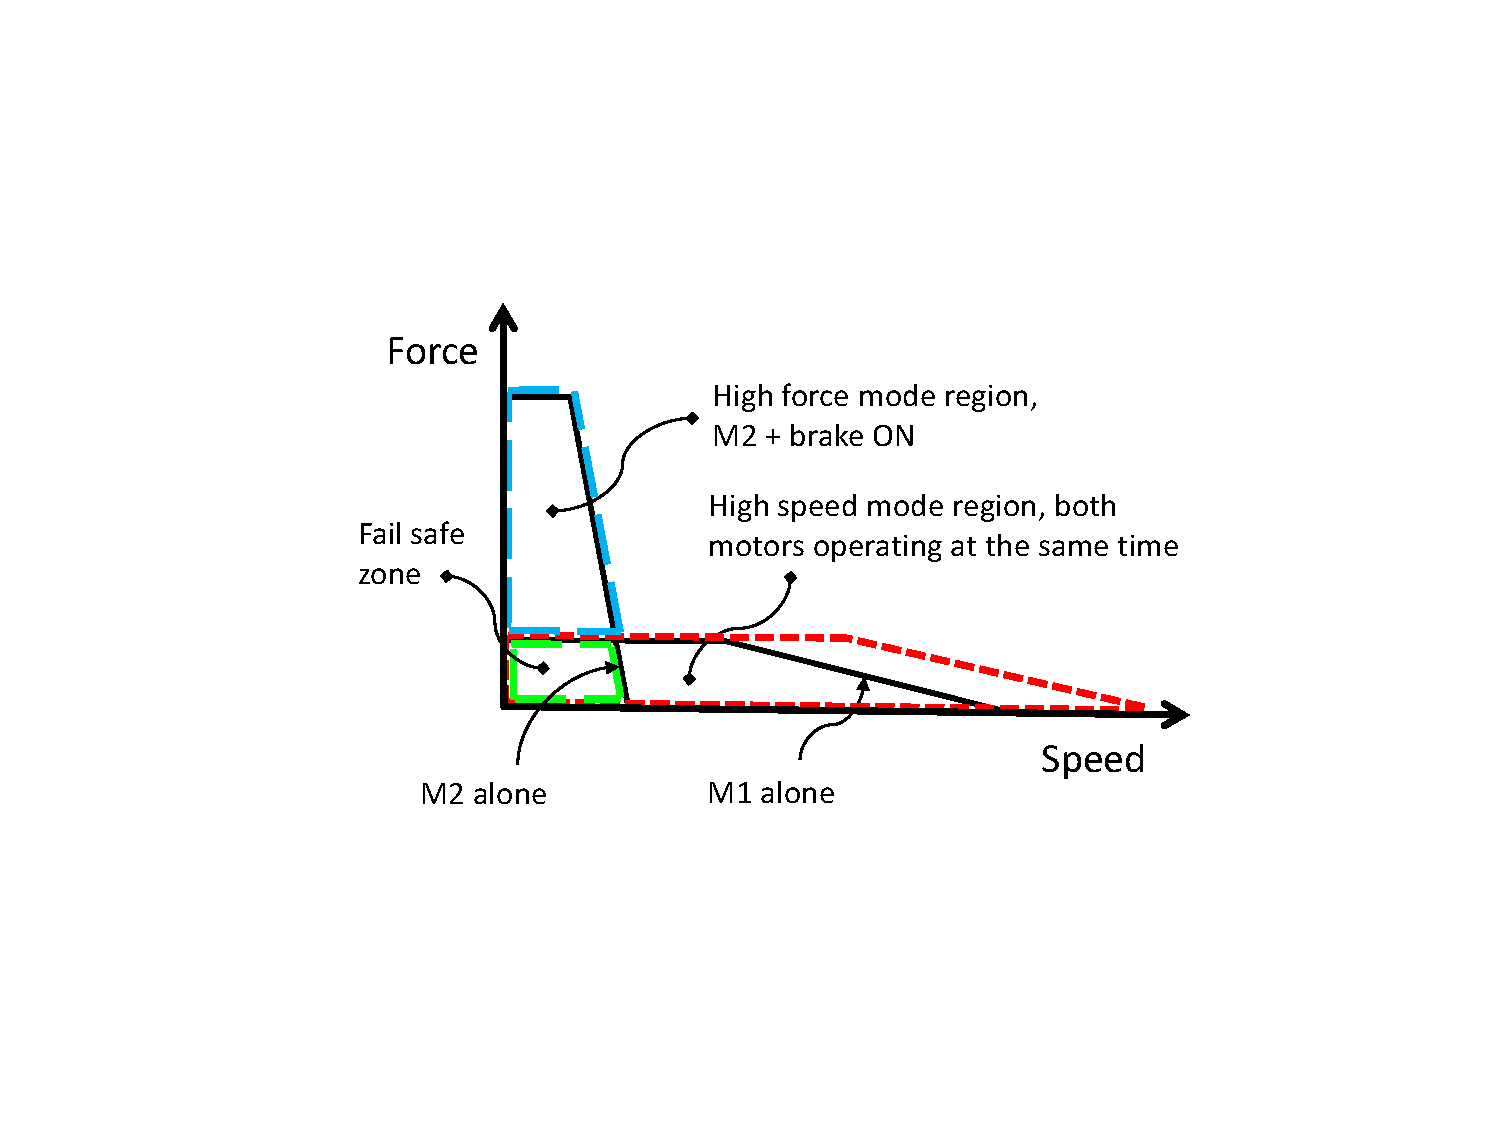
\includegraphics[width=0.65\textwidth]{torquespeed.pdf}
	\caption{DSDM actuator operation region, with a difference between M1 and M2 gearing ratio of only 4 for illustration purposes }
	\label{fig:torquespeed}
\end{figure}

\subsection{Weight advantage}
\label{sec:WeightAdvantage}


A DSDM actuator will be lighter than a single motor for applications with a wide range of operating speed. Suppose that an actuator must generate 10 W output power at two operating points: 0.5 Nm of torque at a speed of 20 rad/sec and 0.1 Nm at 100 rad/sec. A single EM motor that satisfies these requirements at both operating points tends to be oversized in terms of power, to reach both operating points, see Fig. \ref{fig:s1}. A DSDM actuator can reach the same operating points using two smaller motors with appropriate gear ratios, see Fig. \ref{fig:s2}. On the other hand the DSDM actuator uses more components: two motors instead of one, more gearing and an additional brake. The DSDM concept pays-off when the difference in speed between two required operating points becomes larger.  Fig. \ref{fig:1vs2} shows the estimated weight of actuators in relation to the ratio of operating speeds ($\lambda=\frac{w_1}{w_2}$), while the required power output is kept at 10 W. The actuator weight is computed assuming that the mass of each component is proportional to its maximum output torque, with values taken from commercially available components in the 10 - 100 watts range: 2 kg/Nm for motors, 0.1 kg/Nm for gearboxes and differentials and 0.2 kg/Nm for brakes \cite{maxon_motor_usa}. As shown in Fig. \ref{fig:1vs2}, the DSDM concept becomes advantageous when there is a large speed difference between the operating points. This is because only the gearbox and brake need to be scaled up for the DSDM actuator to meet the high torque requirement of the low-speed operating point, while the motor size must be increased for the single motor solution.



\begin{figure}[H]
        \centering
				\subfloat[One motor solution]{
				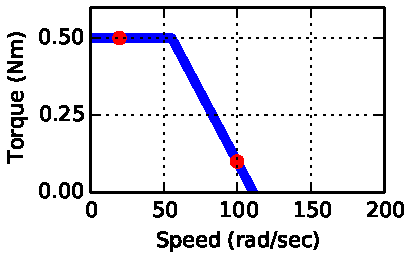
\includegraphics[width=0.42\textwidth]{sol1.pdf}
				\label{fig:s1}}
        \subfloat[DSDM solution]{
				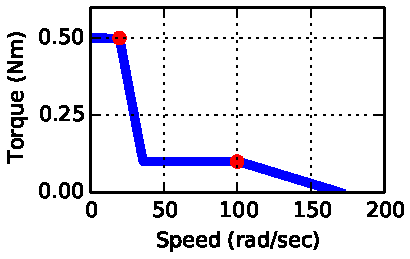
\includegraphics[width=0.42\textwidth]{sol2.pdf}
				\label{fig:s2}}
        \caption{Case study of two actuator solution for two 10 W operating points }\label{fig:solutions}
\end{figure}

\begin{figure}[H]
	\centering
		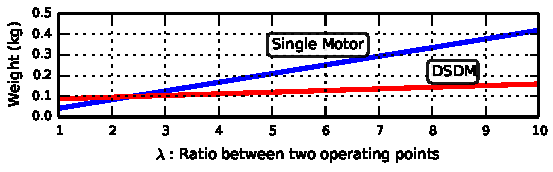
\includegraphics[width=0.75\textwidth]{w_vs_ratio.pdf}
	\caption{Weight of a single motor compared to the DSDM concept for two 10 W operating points at different speeds $w_1=100$ rad/sec, $w_2 = w_1 / \lambda$}
	\label{fig:1vs2}
\end{figure}


\section{Control Algorithms for Fast and Seamless Gearshifts}
\label{sec:FastAndSeamlessGearshifts}

\subsection{Modeling}


\subsubsection{3-ports planetary gear junction}
As illustrated at Fig. \ref{fig:dualmotorconcept} a planetary gear box can be used to implement the differential junction. With the planet carrier connected to the output, M1 to the sun gear and M2 to the ring gear, the kinematic relation of the system is given by
%
\begin{align}
	w_o = 
	\underbrace{ \left[ 
	\frac{ 1 }{N+1}
	\right] }_{  1/R_1  }
	w_1 + 
	\underbrace{ \left[ 
	\frac{ N  }{r_2 (N+1)}
	\right] }_{  1/R_2  }
	w_2
\label{eq:kinematic}
\end{align}
%
where $r_2$ is the additional reduction of M2, $N$ is the ratio of gear teeth of the ring gear over the sun gear, and $w_o$, $w_1$ and $w_2$ are angular velocities of the output shaft (port $o$), M1 input shaft (port $1$) and M2 input shaft (port $2$). Neglecting internal inertial forces in the gearing, the effort relation of the system is given by:
%
\begin{align}
	- e_o =
	\underbrace{ \left[ 
	N+1
	\right] }_{ R_1  }
	e_1 = 
	\underbrace{ \left[ 
	\frac{r_2(N+1)}{N}
	\right] }_{ R_2  }
	e_2
	\label{eq:torque}
\end{align}
%
Hence, the 3-ports planetary coupling can be interpreted as a 0-junction, in the bond graph terminology, with different mechanical advantages ($R_1$ and $R_2$) on each input ports. 

\subsubsection{Dynamics}
\label{sec:dyn}



Fig. \ref{fig:dynamics} shows a lumped-parameter dynamic model of a DSDM when the brake is open (high-speed mode). $J_i$ and $b_i$ are the inertia and damping of the respective i-th ports, $V_1$, $V_2$, $i_1$, $i_2$ are the driving tension and currents in M1 and M2, and $k_m$ is the motor constant. 

\begin{figure}[htb]
	\centering
		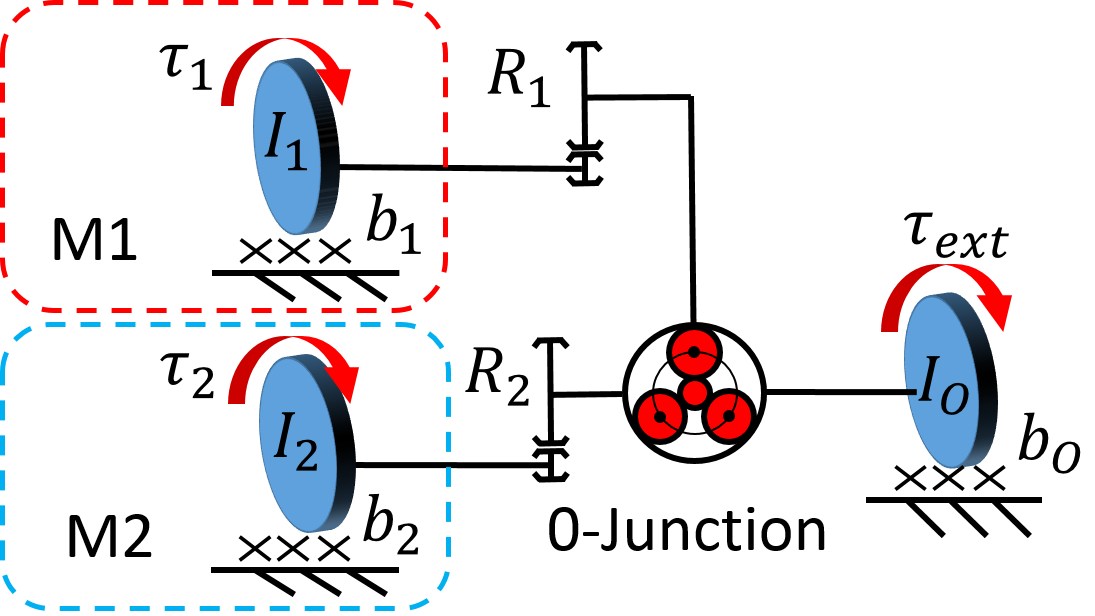
\includegraphics[width=0.65\textwidth]{dynamics.png}
	\caption{Lumped-parameter dynamic model of a DSDM}
	\label{fig:dynamics}
\end{figure}

It is then assumed that low-level high-bandwidth current controller will be used, and electromagnetic torques $\tau_i = k_m i_i$ are going to be considered directly as inputs to the system. Applying Newton's law on each ports yields the following equations of motions:
%
\begin{align}
\tau_{ext}  - e_o &= Z_o(s) w_o \\
\tau_{1}    - e_1 &= Z_1(s) w_1 \\
\tau_{2}    - e_2 &= Z_2(s) w_2
\end{align}
%
where $Z_i(s) = J_i s + b_i$ represents the mechanical impedance of the i-th ports. Note that the system is coupled due to the constraint given by eq. \eqref{eq:kinematic} and \eqref{eq:torque}, and that there is only two degrees of freedom among the three ports. Fig. \ref{fig:dynamics_block}, illustrate the coupled equations motion in block diagram form.

\begin{figure}[htp]
	\centering
		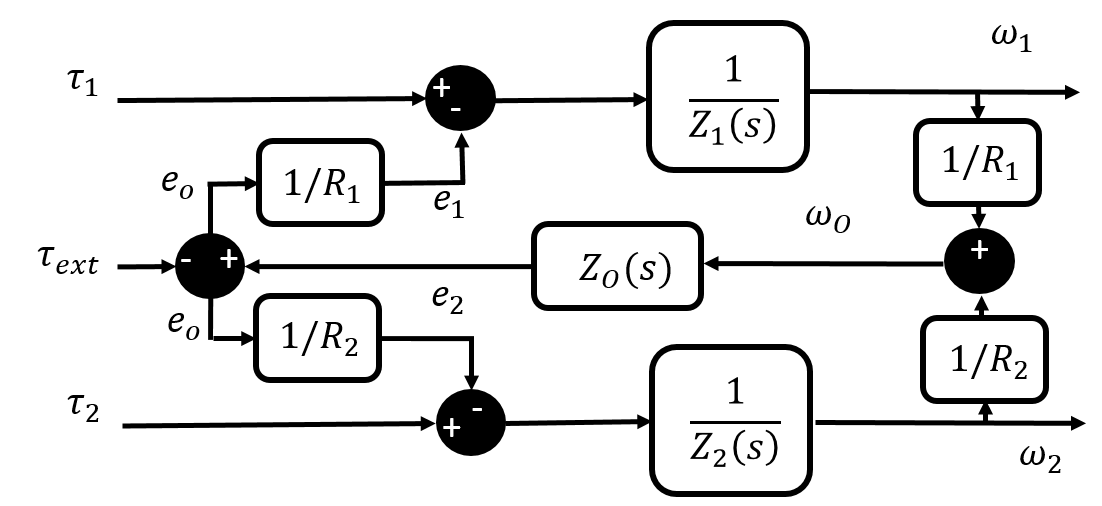
\includegraphics[width=0.60\textwidth]{dynamics_block.png}
	\caption{Dynamics of a DSDM}
	\label{fig:dynamics_block}
\end{figure}

It is then possible to eliminate one variable and express the dynamic as the following system of two equations:
%
\begin{align}
\left[
\begin{array}{c c c}
 1 & 0 & \frac{1}{R_1} \\
 0 & 1 & \frac{1}{R_2}
\end{array}
\right]
\left[
\begin{array}{l}
 \tau_{1} \\
 \tau_{2} \\
 \tau_{ext}
\end{array}
\right]
=
\left[
\begin{array}{c c}
 Z_1(s) + \frac{Z_0(s)}{R_1^2} & \frac{Z_0(s)}{R_1 R_2}        \\
 \frac{Z_0(s)}{R_1 R_2}        & Z_2(s) + \frac{Z_0(s)}{R_2^2} \\
\end{array}
\right]
\left[
\begin{array}{l}
w_1     \\
w_2     \\
\end{array}
\right]
\end{align}
% Alternative
%%
%\begin{align}
%\left[
%\begin{array}{c c c}
 %1 & 0 & \frac{1}{R_1} \\
 %0 & 1 & \frac{1}{R_2}
%\end{array}
%\right]
%\left[
%\begin{array}{l}
 %\tau_{1} \\
 %\tau_{2} \\
 %\tau_{ext}
%\end{array}
%\right]
%=
%\left[
%\begin{array}{c c}
%\frac{Z_o(s)}{R_1}  &   \scriptstyle Z_1(s)   \\
%\frac{Z_o(s)}{R_2}  \scriptstyle + R_2 Z_2(s) & \scriptstyle-\textstyle \frac{R_2}{R_1} \scriptstyle Z_2(s)   \\
%\end{array}
%\right]
%\left[
%\begin{array}{l}
%w_o     \\
%w_1     \\
%\end{array}
%\right]
%\end{align}
%
For more convenience, the equation of motion are then expressed using the output and M1 coordinates ($w_o$ and $w_1$):
%
\begin{align}
\underbrace{ 
\left[
\begin{array}{c c}
 \scriptstyle I_o + R_2^2 I_2           & \scriptstyle - \frac{R_2^2}{R_1} I_2       \\
 \scriptstyle - \frac{R_2^2}{R_1} I_2   & \scriptstyle I_1 + (\frac{R_2}{R_1})^2 I_2  \\
\end{array}
\right] }_{H}
\underbrace{ 
\left[
\begin{array}{l}
\dot{w}_o     \\
\dot{w}_1      \\
\end{array}
\right]}_{\vec{\ddot{q}}}
+
\underbrace{
\left[
\begin{array}{c c}
 \scriptstyle b_o + R_2^2 b_2           & \scriptstyle - \frac{R_2^2}{R_1} b_2       \\
 \scriptstyle- \frac{R_2^2}{R_1} b_2   & \scriptstyle b_1 + (\frac{R_2}{R_1})^2 b_2  \\
\end{array}
\right]
}_{D}
\underbrace{ 
\left[
\begin{array}{l}
w_o     \\
w_1      \\
\end{array}
\right]}_{\vec{\dot{q}}}
=
\underbrace{ 
\left[
\begin{array}{c c c}
 \scriptstyle 0 & \scriptstyle R_2              & \scriptstyle 1 \\
 \scriptstyle 1 & \scriptstyle -\frac{R_2}{R_1} & \scriptstyle 0
\end{array}
\right]}_{B}
\underbrace{
\left[
\begin{array}{l}
 \tau_{1} \\
 \tau_{2} \\
 \tau_{ext}
\end{array}
\right] }_{\vec{\tau}}
\end{align}

The inverse of the inertia matrix is given by:
\begin{align}
H^{-1} = 
\frac{1}{I_o + I_1 R_1 ^2 + I_o \frac{ I_1 }{ I_2 } (\frac{R_1}{R_2})^2}
\left[
\begin{array}{c c}
1 + \frac{ I_1 }{ I_2 } (\frac{R_1}{R_2})^2  & R_1    \\
R_1 & \frac{ I_0 }{ I_2 } (\frac{R_1}{R_2})^2 + R_1^2 \\
\end{array}
\right]
\end{align}

The equations can be converted to linear state space form:
\begin{align}
\underbrace{ \vec{\ddot{q}} }_{\dot{\vec{x}}}
 &= 
\underbrace{ \left[ -H^{-1} D \right] }_{F}
\underbrace{ \vec{\dot{q}} }_{\vec{x}}
+ 
\underbrace{ \left[ H^{-1} B \right] }_{G}
\underbrace{ \vec{\tau} }_{\vec{u}}
\end{align}

Leading to the following after eliminating the external torque and the damping at each motor port for brevity:
\begin{align}
\left[
\begin{array}{c}
\dot{w_o}\\
\dot{w_1}
\end{array}
\right] &= 
\left[
\begin{array}{c c}
\frac{-b_T}{I_T} &   0 \\
\frac{-R_1 b_o}{I_T}  &  0 \\
\end{array}
\right]
\left[ \begin{array}{c}
w_o \\
w_1
\end{array} \right]+
\underline{G}
\left[ \begin{array}{c}
\tau_1 \\
\tau_2
\end{array} \right] 
\label{eq:ss}
\\
\text{with} \quad 
\underline{G} &= 
\frac{1}{I_T}
\left[
\begin{array}{c c}
 R_1  &   R_1 \frac{R_1 I_1}{R_2 I_2}  \\
(R_1^2+\frac{R_1^2 I_o}{R_2^2 I_2})  &  - \frac{R_1 I_o}{R_2 I_2} \\
\end{array}
\right] \\
 I_T &=  \scriptstyle \left[   I_o + R_1^2 I_1 + \left( \frac{R_1}{R_2} \right)^2 \frac{I_1}{I_2} I_o \right]\\
 b_T &= \scriptstyle \left[ b_o + \left( \frac{R_1}{R_2} \right)^2 \frac{I_1}{I_2} b_o \right] 
\end{align}
%


\subsubsection{Inputs/Outputs equations}
\label{sec:out}

The variable of interest is the output $w_o$, and its dynamic can be expressed, going back to the Laplace domain by:
%
\begin{align}
\left[
 Z_1(s) Z_2(s) + \frac{Z_1(s) Z_o(s)}{R_2^2} + \frac{Z_2(s) Z_o(s)}{R_1^2}
\right] w_o(s) = \\
\left[
 \frac{Z_2(s)}{R_1}
\right] \tau_1(s)  + 
\left[
 \frac{Z_1(s)}{R_2}
\right] \tau_2(s)  + 
\left[
 \frac{Z_2(s)}{R_1^2} + \frac{Z_1(s) }{R_2^2}
\right] \tau_{ext}(s)
\label{eq:dsdm_output}
\end{align}

When the brake on M1 of the DSDM is locked, the output equation is reduced, by letting $Z_1(s) \rightarrow \infty$, to:
\begin{align}
\left[
 Z_o(s)  + R_2^2 Z_2(s)
\right] w_o(s) = 
\left[
R_2
\right] \tau_2(s)  + 
\tau_{ext}(s)
\label{eq:dsdm_output_HF}
\end{align}

When the brake is open, if the gear-ratio $R_2$ of M2 is large, the equation can be simplified. 
%
%, the behavior can be approximated. First eq. \eqref{eq:dsdm_output} is rearranged:
%\begin{align}
%\left[
%\scriptstyle Z_1(s) R_1^2 + \left(1 + \frac{Z_1(s) R_1^2 }{ Z_2(s) R_2^2} \right) Z_o(s)
%\right] w_o(s) = 
%\left[
%R_1
%\right] \tau_1(s)  + 
%\left[
%\scriptstyle R_1 \frac{R_1 Z_1(s)}{R_2 Z_2(s)}
%\right] \tau_2(s)  + 
%\left[
%\scriptstyle  1 + \frac{Z_1(s) R_1^2 }{ Z_2(s) R_2^2} 
%\right] \tau_{ext}(s)
%\label{eq:dsdm_output_HS}
%\end{align}
%
Assuming the reflected impedance of M1 is much smaller than that of M2, and neglecting motor side damping, the equation reduce to:
\begin{align}
\left[
Z_o(s)  + R_1^2 Z_1(s)
\right] w_o(s) &= 
\left[
R_1
\right] \tau_1(s)  + 
\left[
R_1 \frac{R_1 I_1}{R_2 I_2}
\right] \tau_2(s)  + 
\tau_{ext}(s) \\
&\text{if} \quad Z_1(s) R_1^2 << Z_2(s) R_2^2 
\quad \& \quad \frac{Z_1(s)}{Z_2(s)} = \frac{I_1}{I_2}
\label{eq:dsdm_output_HF}
\end{align}

During high-speed mode the behavior of the output is also dominated by a first-order linear behavior, but interestingly both input torques contributed to the motion through inertial coupling. Note that this differ from a serial architecture, in both case speed adds-up and effort is shared (0-type junction), but inertial properties are different.


\subsubsection{Discrete Operating Modes}

Fig. \ref{fig:operatingmodes} illustrates the different discrete operating modes of the system. During high-force mode, when the brake is engaged, the actuator only has a single DoF and control input and the dynamic behavior is described by the Laplace transfer function given by eq. \eqref{eq:dsdm_output_HF}. During high-speed mode, when the brake is open, the actuator has two DoF and two control inputs and the dynamic behavior is described by state space equation given by eq. \eqref{eq:ss}.

\begin{figure}[H]
	\centering
		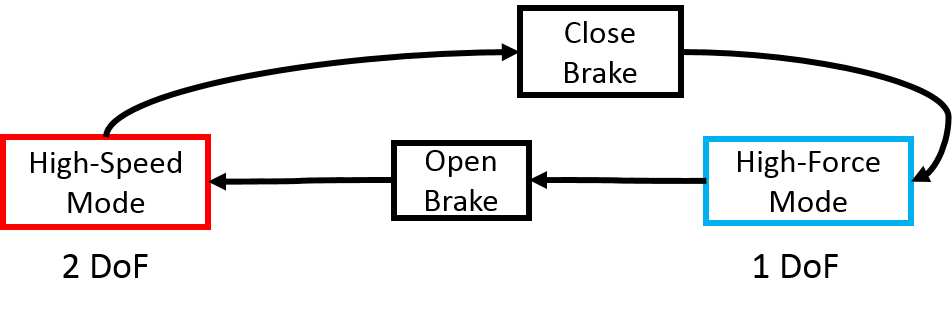
\includegraphics[width=0.65\textwidth]{operating_modes.png}
	\caption{Discrete operating modes of the actuators}
	\label{fig:operatingmodes}
\end{figure}



\subsection{Nullspace of the system}

During high-speed mode, from the kinematic input-output view point, the DSDM actuator has one redundant degree of freedom. In other words, there is an infinite number of combinations of $w_1$ and $w_2$ producing the same output speed $w_0$, from eq.\eqref{eq:kinematic}:  
%
\begin{align}
\left[
w_o
\right] = 
\left[
\begin{array}{c c}
\frac{1}{R_1} & \frac{1}{R_2}
\end{array}
\right]
\left[
\begin{array}{c}
w_1 \\
w_2 \\
\end{array}
\right]
\end{align}
%
A vector perpendicular to the above coefficient vector forms the null space of the DSDM actuator system. Any input combination in this direction produces zero output speed:
%
\begin{align}
\left[
\begin{array}{c}
w_1 \\
w_2 \\
\end{array}
\right]=
\underbrace{\left[
\begin{array}{c}
1 \\
-R_2/R_1 \\
\end{array}
\right]}_{\text{Nullspace Projection}}
u  \; \rightarrow \;
w_0 = 0 \quad \forall u \in \Re
\label{eq:kinematicnullspace}
\end{align}
%
Interestingly, a similar expression can be obtained for the dynamics of the output in response to electromagnetic torque inputs, from the first line of eq.\eqref{eq:ss}:
%
\begin{align}
I_T \dot{w}_o +
b_T  w_o
=&
\left[ \begin{array}{c c}
R_1 & R_1 \frac{R_1 I_1}{R_2 I_2}
\end{array} \right]
\left[ \begin{array}{c}
\tau_1 \\
\tau_2
\end{array} \right]
\label{eq:output}
\end{align}
% 
Hence, there is a one degree of freedom space of inputs $\tau_1$ and $\tau_2$ that do not affect the output:
\begin{align}
\left[ \begin{array}{c}
\tau_1 \\
\tau_2
\end{array} \right]
 = 
\underbrace{\left[ \begin{array}{c}
1 \\
-\frac{R_2 I_2}{R_1 I_1} 
\end{array} \right]}_{\text{Nullspace Projection}} u
\; \rightarrow \;
I_T \dot{w}_o +
b_T  w_o = 0 \quad \forall u \in \Re
\label{eq:dyn_null_proj}
\end{align}



\subsection{Control algorithms}

During high-force mode, the actuator behaves like a regular geared EM motor and standard speed or position control scheme can be used. During high-speed mode, with a small reduction ratio $R_1$ (high transparency transmission), the DSDM actuator can be controlled like a direct drive motor: controlling M1 current lead to almost direct control of the output torque. Moreover, exploiting the nullspace, a secondary objective can be brought into the system without influencing the output torque. In case the first motor is overloaded, for example, the second motor can reduce the load by projecting inputs through the null space, producing no effect upon the output, but changing the proportion of the two input commands. The secondary controller can be used not only for load balancing but also for minimizing power consumption, avoiding speed saturation of M1, etc. Note that the nullspace projection vector, see eq.\eqref{eq:dyn_null_proj}, depends only on parameters associated with the motors. Therefore, it is possible to project the secondary controller inputs on the output nullspace even if the output dynamic parameters that include the load inertia and damping are unknowns. 

Fig. \ref{fig:HS_loop} and Fig. \ref{fig:HF_loop} show DSDM control algorithms implemented as intermediary control loops between hardware and high-level commands. The high-speed controller tracks a received desired torque by controlling the current in M1, and can also optionally track a secondary objective without affecting the main-loop, by projecting the secondary input into the nullspace of the main-loop. The high-force controller directly convert a received desired torque to a current set-point for M2.

%The high-level robot controller, discussed in detail in Chapter \ref{sec:ControlAndPlanningOfRobotUsingVariableGearRatioActuators}, could be a simple PID for a single output system, a computed torque algorithm for a complex robots, etc. 
 

\begin{figure}[p]
	\centering
		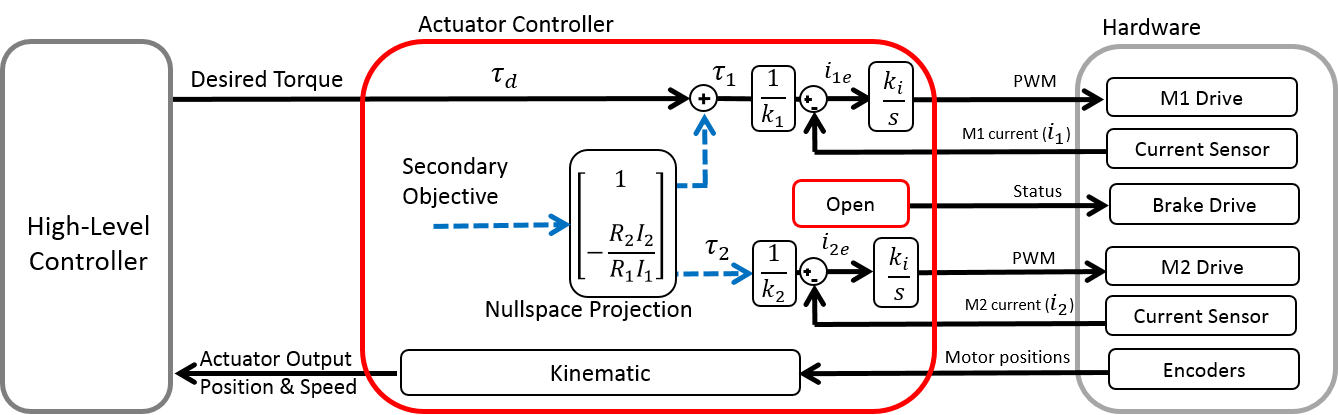
\includegraphics[width=0.95\textwidth]{HS_ctl.png}
	\caption{High-speed mode control loop}
	\label{fig:HS_loop}
\end{figure}

\begin{figure}[p]
	\centering
		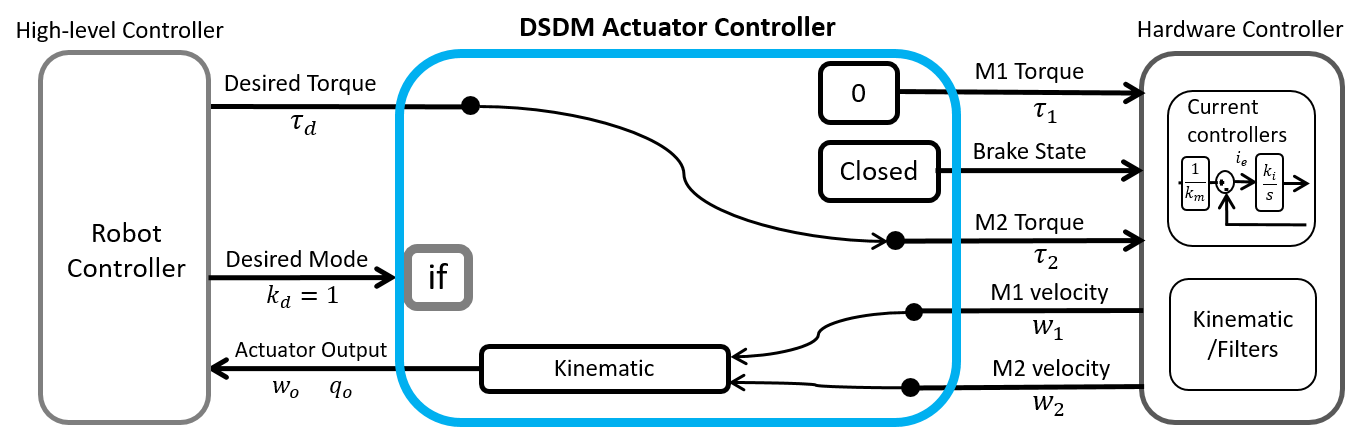
\includegraphics[width=0.95\textwidth]{HF_ctl.png}
	\caption{High-force mode control loop}
	\label{fig:HF_loop}
\end{figure}

\begin{figure}[p]
	\centering
		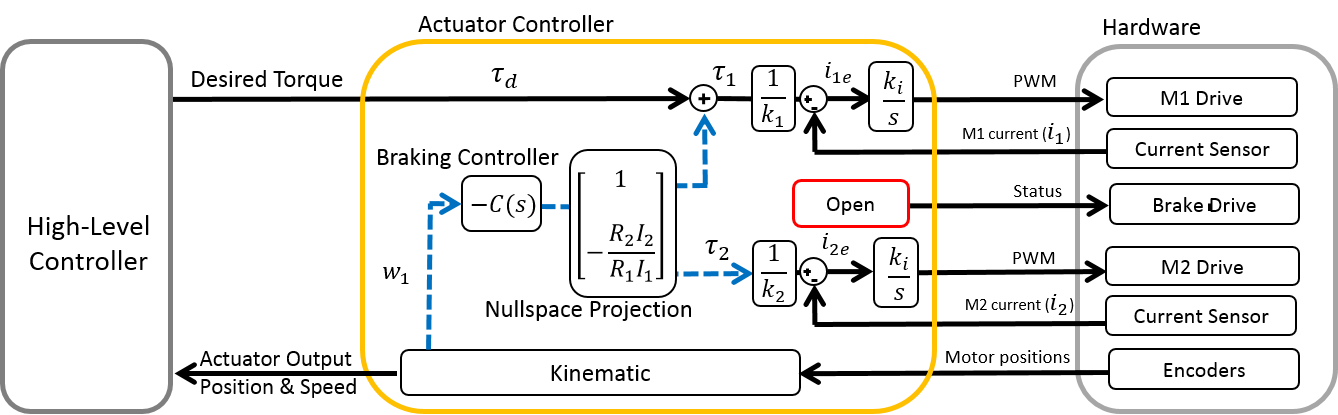
\includegraphics[width=0.95\textwidth]{down_ctl.png}
	\caption{Synchronization mode control loop}
	\label{fig:down_loop}
\end{figure}




\subsubsection{Transitions (gear-shift)}

This section addresses transition control between the two discrete operating modes. Fig. \ref{fig:automaticflow} show the state machine used to transit between the different necessary control mode.

\begin{figure}[H]
	\centering
		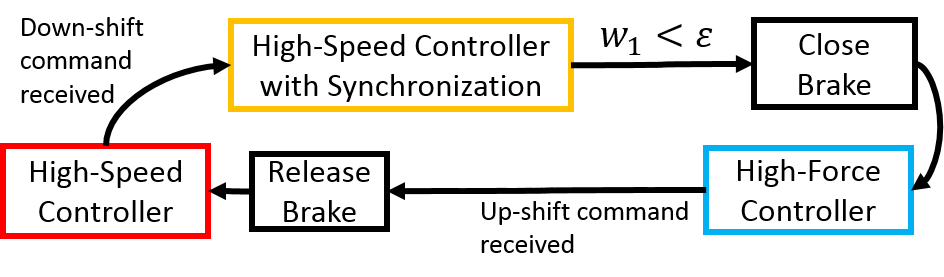
\includegraphics[width=0.70\textwidth]{discrete_control_modes.png}
	\caption{State machine of discrete control modes}
	\label{fig:automaticflow}
\end{figure}


\paragraph{Up-shift: From high-force mode to high-speed mode}
In this case, the transition is simple because the system goes from 1 DoF to 2 DoF. The locking brake can be released anytime, M1 is then instantaneously freed and the controller can immediately switch to the high-speed control mode.
%

\paragraph{Down-shift: From high-speed mode to high-force mode}
In this case, the transition is harder because the system goes from 2 DoF to 1 DoF, and some synchronization work is needed. M1 speed $w_1$ must be brought to zero so that the locking brake can be engaged smoothly without any impact. Hence, as illustrated at Fig. \ref{fig:automaticflow}, when it is decided to engage high-force mode, and intermediary synchronization control mode is needed. Two algorithms, a kinematic and a dynamic approach, can be considered. The former assumes local high gain velocity feedback controls for the individual motors. Hence velocities $w_1$ and $w_2$ can be treated as control inputs. Using the nullspace projection vector from eq.\eqref{eq:kinematicnullspace}, the kinematic control law can be written as 
%
\begin{align}
\left[
\begin{array}{c}
w_1 \\
w_2 \\
\end{array}
\right]=
\underbrace{\left[
\begin{array}{c}
1 \\
-R_2/R_1 \\
\end{array}
\right]}_{\text{Nullspace Projection}}
u_1 + 
\left[
\begin{array}{c}
0 \\
R_2 \\
\end{array}
\right] u_2
\label{eq:kinematicsys}
\end{align}
%
leading to
%
\begin{align}
w_o = u_2 \quad \text{with} \quad w_1 = u_1
\end{align}
%
Therefore during transitions, using $u_1$ velocity $w_1$ can be driven to zero, while fully controlling the output velocity using $u_2$. The kinematic control law is valid only when high fidelity velocity controls are available. Alternatively the dynamic control algorithm does not require this. As illustrated in Fig. \ref{fig:down_loop}, while running the general high-speed controller, a braking law for $w_1$ can be used in parallel as the secondary controller projected on the output nullspace:
\begin{align}
\left[ \begin{array}{c}
\tau_1 \\
\tau_2
\end{array} \right]
 = 
\underbrace{\left[ \begin{array}{c}
1 \\
-\frac{R_2 I_2}{R_1 I_1} 
\end{array} \right]}_{\text{Nullspace Projection}} \underbrace{-C w_1}_{\text{Braking Law}} + 
\left[ \begin{array}{c}
\frac{1}{R_1} \\
0 
\end{array} \right]  \tau_d
\end{align}
leads  to:
\begin{align}
I_T \dot{w}_o +
b_T  w_o
=& \, \tau_d  \quad \text{and} \quad \dot{w}_1 = -C w_1 + f(w_o,\tau_d) %\scriptstyle \frac{R_1 b_o}{I_T} \textstyle w_o
\end{align}
Hence, the output is not influenced by the braking law due to orthogonality, and is still controlled using the desired torque $\tau_d$ determined by the high-speed mode controller. On the other hand, $w_1$ is directly influenced by the braking law but also by the output speed and the desired output torque $\tau_d$. Mathematically, it would be possible to also fully uncouple $\dot{w}_1$ equation, but the control law would not be practical in the scenario of $R_1<<R_2$ when considering torque and speed saturations. Increasing the gain $C$ will lead to faster braking of $w_1$, however motor torque will saturate if the gain is too large. A large $C$ can still be used for faster braking at a cost of deviation from the desired torque $\tau_d$. There is a trade-off, passed the torque saturation point, between fast braking of $w_1$ for fast transition and high-fidelity output torque control.



\subsubsection{Leveraging Impact Forces}

DSDM model with impulsive force only:


generalized coords:

%
\begin{align}
\vec{\dot{q}} = \left[ \begin{array}{c} 	\dot{a} \\ w_1 \end{array} \right]
\label{eq:dsdm_impact_q}
\end{align}
%


%
\begin{align}
H = \left[ \begin{array}{c c} 	m_0 + R_1^2 I_1  &  -\frac{R_1^2}{R_2} I_1 \\ -\frac{R_1^2}{R_2} I_1  &  I_1 + (\frac{R_2}{R_1})^2 I_2 \end{array} \right]
\label{eq:dsdm_impact_H}
\end{align}
%

constraint
%
\begin{align}
\dot{a} &= 0 \\
J_c     &= \left[ \begin{array}{c c} 1 & 0 \end{array} \right]
\label{eq:dsdm_impact_const}
\end{align}
%

%
\begin{align}
J_c     &= \left[ \begin{array}{c c} 1 & 0 \end{array} \right] \\ 
V       &= \left[ \begin{array}{c} 0 \\ 1 \end{array} \right]
\label{eq:dsdm_impact_jaco}
\end{align}
%


Then solving for a sticky impact, see section \ref{sec:impact}:

%
\begin{align}
\left[ \begin{array}{c} \lambda \\ \int{f_c dt} \end{array} \right] &= \Bigg[ \begin{array}{c c} HV & -J_c^T \end{array} \Bigg]^{-1} \Bigg[ H \Bigg] \left[ \begin{array}{c} \dot{a}^- \\ \dot{w}_1^- \end{array} \right] \\
\left[ \begin{array}{c} \lambda \\ \int{f_c dt} \end{array} \right] &= \Bigg[ \begin{array}{c c} 
\frac{-R_2^2/R_1 J_2}{J_1+(\frac{R_1}{R_2})^2 J_2} & 1 \\
- (m_o + R_2^2 J_2+\frac{-R_2^2/R_1 J_2}{J_1+(\frac{R_1}{R_2})^2 J_2}) & 0 
\end{array} \Bigg] \left[ \begin{array}{c} \dot{a}^- \\ \dot{w}_1^- \end{array} \right]
\label{eq:dsdm_impact_sol}
\end{align}
%

Then simplifying for the case of $(\frac{R_2}{R_2})^2 J_2 >> J_1 $ we have the following results:
%
\begin{align}
\dot{a}^+ &= 0 \\
w_1^+     &\approx - R_1 \dot{a}^- + w_1^-  = - \frac{R_1}{R_2} w_2^- \\
w_2^+     &\approx  w_2^- \\
\int{f_c dt}     &\approx -[m_o + R_1^2 J_1] \dot{a}^-
\label{eq:dsdm_impact_res}
\end{align}
%

Those results basically show that when the reflected inertia of M2 is much greater than that of M1, the impact affect only $w_1$ and $w_2$ remains unchanged. 

Interestingly 

